% !Mode:: "TeX:UTF-8"
% !TEX program  = xelatex
\documentclass[a4paper]{article}
\usepackage{amsmath}
\usepackage{amssymb}
\usepackage{ctex}
%\usepackage{braket}
%\usepackage[european]{circuitikz}
\usepackage{multirow}
\usepackage{float}
\usepackage{colortbl}
\usepackage{graphicx}
\usepackage{geometry}
\geometry{left=2.5cm,right=2.5cm,bottom=2.5cm,top=2.5cm}
\title{近代物理实验报告3.1:椭偏光法测量薄膜的厚度和折射率}
\author{xy\quad 学号\quad 匡亚明学院}
\date{2019年2月29日}
\begin{document}
\maketitle
\bibliographystyle{unsrt}
%--------main-body------------

\section{引言}
椭圆偏振测量法,简称椭偏光法,是测量研究介质表面界面或薄膜光学特性的一种重要光学方法。它是将一束偏振光非垂直地投射到被测样品表面,有由观察反射光或透射光的偏振状态的变化来推知样品的光学特性。例如薄膜的厚度,材料的复折射率等。这种测量方法的有点是测量精度非常高,而且对样品是非破坏性的,它可以测量出薄膜厚度约0.1nm的变化。因此可以用于表面界面的研究。也可用于准单原子层开始的薄膜生长过程的实时自动检测。

椭偏光法的应用范围广泛,自然界中普遍存在各种各样的薄膜和i二面,人工制备薄膜的种类也越来越多,因此椭偏光法应用于物理、化学、表面科学、材料科学、生物科学以及有关光学、微电子、机械、冶金和生物医学等领域中。在材料科学中椭偏测量常用来测量各种功能介质薄膜、硅上超薄氧化层以及超薄异质层生长的实时监控、溅射过程的实时监控等。

自1945年罗申(A. Rothen)描述了用以测量薄膜表面光学性质的椭偏仪来,随着科学技术的迅速发展,椭偏光法发展很快,椭偏仪的制造水平也不断提高,特别是使用计算机处理复杂繁冗的而太平洋测量数据后使测量快捷简便了许多。

\section{实验目的}
\begin{enumerate}
\item 了解椭偏光法测量原理和实验方法。
\item 熟悉椭偏光仪器的结构和调试方法。
\item 测量介质薄膜样品的厚度和折射率,以及硅的消光系数和复折射率。
\end{enumerate}

\section{实验仪器}
椭圆偏振仪。本实验使用的手动型椭偏仪(TP-77型)如图(!椭偏仪!)所示一起采用632.8nm的波长He-Ne激光器作为单色光源,入射角和反射角均在90$^{\circ}$内自由调节,样品台可绕纵轴旋转,其高度和水平可以调节。检偏器旁边有一个观察窗,窗下的旋钮用以改变经检偏器出射的光或射向观察窗或射向光电倍增管。为了保护光电倍增管,该旋钮应经常放在观察窗位置。

\section{实验原理}
本实验介绍反射型椭偏光测量方法。其基本原理是用一束椭偏光照射在薄膜样品上,光在介质膜的交界面发生多次反射和折射,反射光的振幅和相位发生变化,这些变化与薄膜的厚度和光学参数(折射率、消光系数等)有关,因此只要测处反射光偏振状态的变化,就可以推出薄膜的厚度和折射率等。

\subsection{椭圆偏振方程}
在一光学材料上镀各向同性的单层介质膜后,光线的反射和折射在一般情况下会同时存在的。 通常,设介质层为$n_1$、$n_2$、$n_3$,$\phi_1$为入射角,那么在1、2介质交界面和 2、3介质交界面会产生反 射光和折射光的多光束干涉,如图1。

\begin{figure}[!h]
\centering
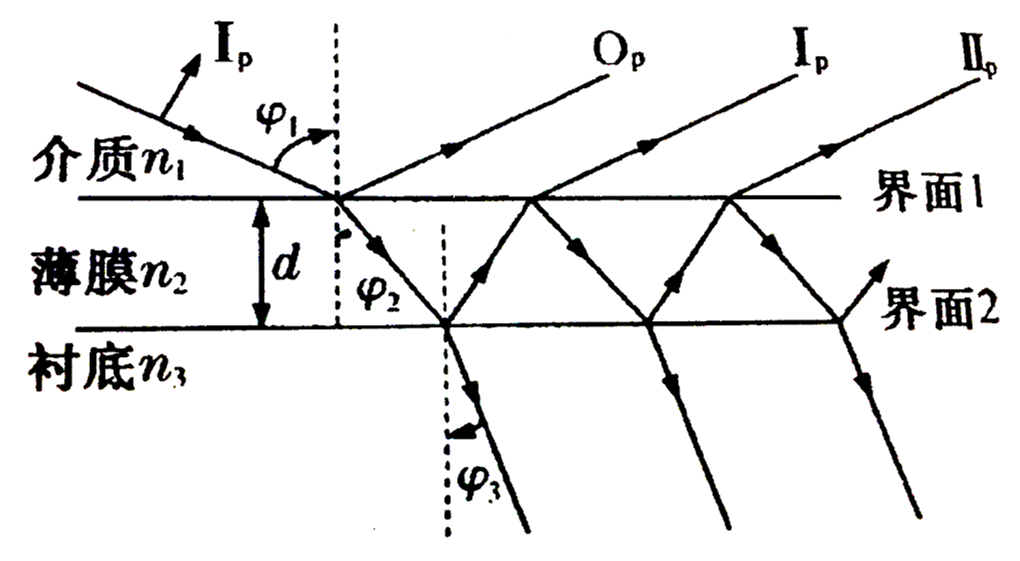
\includegraphics[width = 0.5\textwidth]{fig/1.png}
\caption{多光束干涉示意图}
\end{figure}

这里我们用$2\delta$表示相邻两分波的相位差,其中$\delta=\frac{2\pi dn_2}{\lambda}\cos\phi_2$,用 $r_{1p}$、$r_{1s}$ 表示光线的p分量、 s 分量在界面 1、 2间的反射系数,用	$r_{2p}$  、 $r_{2s}$ 表示光线的p分量、 s 分量在界面 2、 3间的反射系数。由多光束干涉的复振幅计算可知:
$$E_{rp}=\frac{r_{1p}+r_{2p}{\rm e}^{-i2\delta}}{1+r_{1p}r_{2p}{\rm e}^{-i2\delta}}E_{ip},$$
$$E_{rs}=\frac{r_{1s}+r_{2s}{\rm e}^{-i2\delta}}{1+r_{1s}r_{2s}{\rm e}^{-i2\delta}}E_{is}.$$
其中 $E_{ip}$  和 $E_{is}$ 分别代表入射光波电矢量的	p 分量和 s 分量, $E_{rp}$ 和 $E_{rs}$ 分别代表反射光波电矢量的 p 分量和 s 分量。现将上述	$E_{ip}$ 、$E_{is}$ 、$E_{rp}$、 $E_{rs}$ 四个量写成一个量$G$,即:
$$G=\frac{E_{rp}/E_{rs}}{E_{ip}/E_{is}}=\tan\Psi{\rm e}^{i\Delta}=\frac{r_{1p}+r_{2p}{\rm e}^{-i2\delta}}{1+r_{1p}r_{2p}{\rm e}^{-i2\delta}} \frac{r_{1s}+r_{2s}{\rm e}^{-i2\delta}}{1+r_{1s}r_{2s}{\rm e}^{-i2\delta}}.$$
我们定义	$G$ 为反射系数比,它应为一个复数,可用$\tan\Psi$和 $\Delta$ 表示它的模和幅角。上述公式的过程量转换可由菲涅耳公式和折射公式给出:
$$\left\{
\begin{aligned}
&r_{1p}=(n_2\cos\phi_1-n_1\cos\phi_2)/(n_2\cos\phi_1+n_1\cos\phi_2)\\
&r_{2p}=(n_3\cos\phi_2-n_2\cos\phi_3)/(n_3\cos\phi_2+n_2\cos\phi_3)\\
&r_{1s}=(n_1\cos\phi_1-n_2\cos\phi_2)/(n_1\cos\phi_1+n_2\cos\phi_2)\\
&r_{2s}=(n_2\cos\phi_2-n_3\cos\phi_3)/(n_2\cos\phi_2+n_3\cos\phi_3)\\
&2\delta=4\pi dn_2\cos\phi_2/\lambda\\
&n_1\cos\phi_1=n_2\cos\phi_2=n_3\cos\phi_3\end{aligned}\right.$$

$G$是变量 $n_1$、 $n_2$、 $n_3$、 $d$、 $\lambda$ 、$\phi_1$的函数 ($\phi_2$ 、 $\phi_3$可用 $\phi_1$表示 ) ,即$\Psi=\tan^{-1}f$ , $\Delta=\arg|f|$, 称 $\Psi$ 和$\Delta$ 为椭偏参数,上述复数方程表示两个等式方程:
$$\textbf{Re}\{\tan\Psi{\rm e}^{i\Delta}\}=\textbf{Re}\left\{\frac{r_{1p}+r_{2p}{\rm e}^{-i2\delta}}{1+r_{1p}r_{2p}{\rm e}^{-i2\delta}} \frac{r_{1s}+r_{2s}{\rm e}^{-i2\delta}}{1+r_{1s}r_{2s}{\rm e}^{-i2\delta}}\right\}$$
$$\textbf{Im}\{\tan\Psi{\rm e}^{i\Delta}\}=\textbf{Im}\left\{\frac{r_{1p}+r_{2p}{\rm e}^{-i2\delta}}{1+r_{1p}r_{2p}{\rm e}^{-i2\delta}} \frac{r_{1s}+r_{2s}{\rm e}^{-i2\delta}}{1+r_{1s}r_{2s}{\rm e}^{-i2\delta}}\right\}$$

若能从实验测出$\Psi$ 和$\Delta$ 的话, 原则上可以解出$n_2$和 $d$ ($n_1$、$n_3$、$\lambda$ 、$\phi_1$已知 ),根据公式 (4)$\sim$(9) , 推导出 $\Psi$ 和 $\Delta$与 $r_{1p}$、 $r_{1s}$、 $r_{2p}$、 $r_{2s}$、和 $\delta$的关系:
$$\tan\Psi=\left[\frac{r_{1p}^2+r_{2p}^2+2r_{1p}r_{2p}\cos2\delta}{1+r_{1p}^2r_{2p}^2+2r_{1p}r_{2p}\cos2\delta} \cdot \frac{1+r_{1s}^2r_{2s}^2+2r_{1s}r_{2s}\cos2\delta}{r_{1s}^2+r_{2s}^2+2r_{1s}r_{2s}\cos2\delta}\right]^{1/2},$$
$$\Delta=\tan^{-1}\frac{-r_{2p}(1-r_{1p}^2)\sin2\delta}{r_{1p}(1+r_{2p}^2)+r_{2p}(1+r_{1p}^2)\cos2\delta} - \tan^{-1}\frac{-r_{2s}(1-r_{1s}^2)\sin2\delta}{r_{1s}(1+r_{2s}^2)+r_{2s}(1+r_{1s}^2)\cos2\delta}$$

由上式经计算机运算,可制作数表或计算程序。这就是椭偏仪测量薄膜的基本原理。若	$d$ 是已知, $n_2$为复数的话,也可求出$n_2$的实部和虚部。那么,在实验中是如何测定$\Psi$ 和 $\Delta$ 的呢?现用复数 形式表示入射光和反射光:
$$\widetilde{E}_{ip}=|E_{ip}|{\rm e}^{i\beta_{ip}},\widetilde{E}_{is}=|E_{is}|{\rm e}^{i\beta_{is}},\widetilde{E}_{rp}=|E_{rp}|{\rm e}^{i\beta_{rp}},\widetilde{E}_{rs}=|E_{rs}|{\rm e}^{i\beta_{rs}}$$
所以:
$$G=\tan\Psi{\rm e}^{i\Delta}=\frac{|E_{rp}/E_{rs}|}{|E_{ip}/E_{is}|}{\rm e}^{i((\beta_{rp}-\beta_{rs})-(\beta_{ip}-\beta_{is}))}$$
其中:
$$\tan\Psi=\frac{|E_{rp}/E_{rs}|}{|E_{ip}/E_{is}|},$$
$${\rm e}^{i\Delta}={\rm e}^{i((\beta_{rp}-\beta_{rs})-(\beta_{ip}-\beta_{is}))}.$$
这时需测四个量, 即分别测入射光中的两分量振幅比和相位差及反射光中的两分量振幅比和相位差, 如设法使入射光为等幅椭偏光,	$E_{ip}/E_{is} = 1$ ,则 $\tan\Psi=|E_{rp}/E_{rs}|$;对于相位角,有:
$$\Delta=(\beta_{rp}-\beta_{rs})-(\beta_{ip}-\beta_{is})\Rightarrow\Delta+\beta_{ip}-\beta_{is}=\beta_{rp}-\beta_{rs}.$$
因为入射光 $\beta_{ip}$ 和$\beta_{is}$ 连续可调,调整仪器,使反射光成为线偏光,即	$\beta_{rp}-\beta_{rs}=0\text{或}\pi$,则$\Delta=-(\beta_{ip}- \beta_{is})$或$\Delta=\pi-(\beta_{ip}-\beta_{is})$,可见$\Delta$只与反射光的 p 波和 s 波的相位差有关, 可从起偏器的方位 角算出。对于特定的膜, $\Delta$ 是定值,只要改变入射光两分量的相位差$ (\beta_{ip}- \beta_{is})$,肯定会找到特定值 使反射光成线偏光, $\beta_{rp}-\beta_{rs}=0\text{或}\pi$.

\subsection{实际检测方法}
等幅椭圆偏振光的获得	(实验光路如图	2),平面偏振光通过四分之一波片,使得具有$\pm\pi/4$相位 差,使入射光的振动平面和四分之一波片的主截面成45$^{\circ}$。
\begin{figure}[!h]
\centering
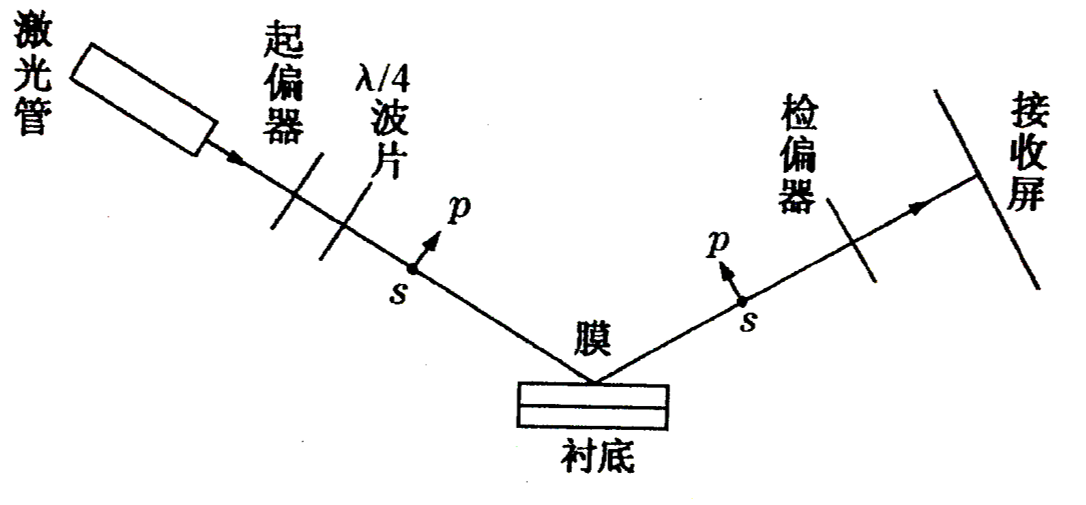
\includegraphics[width = 0.7\textwidth]{fig/2.png}
\caption{椭偏测厚仪光路图}
\end{figure}
\subsection{反射光的检测}
将四分之一波片置于其快轴方向$f$ 与 $x $方向的夹角 $\alpha$为$\pi/4$的方位, $E_0$ 为通过起偏器后的电矢量, $P$ 为 $E_0$与 $x$ 方向间的夹角。通过四分之一波片后,	$E_0$ 沿快轴的分量与沿慢轴的分量比较,相位上超前$\pi/2$。
$$\left\{\begin{aligned}&E_f=E_0{\rm e}^{i\pi/2}\cos(P-\pi/4)\\
&E_s=E_0\sin(P-\pi/4)\end{aligned}\right.$$
在 $x$ 轴、 $y$ 轴上的分量为:
$$E_x=E_f\cos\pi/4-E_s\sin\pi/4=\frac{\sqrt2}{2}E_0{\rm e}^{i\pi/2}{\rm e}^{i(P-\pi/4)},$$
$$E_y=E_f\sin\pi/4+E_s\cos\pi/4=\frac{\sqrt2}{2}E_0{\rm e}^{i\pi/2}{\rm e}^{-i(P-\pi/4)}.$$

由于 $x$ 轴在入射面内,而	$y$ 轴与入射面垂直,故$E_x$ 就是 $E_{ip}$, $E_y$ 就是 $E_{is}$。
$$E_{ip}=\frac{\sqrt2}{2}E_0{\rm e}^{i(\pi/4+P)},$$
$$E_{rp}=\frac{\sqrt2}{2}E_0{\rm e}^{-i(\pi/4+P)}.$$

由此可见,当$\alpha=\pi/4$时,入射光的两分量的振幅均为	$E_0/\sqrt2$,它们之间的相位差为$2P-\pi/2$	, 改变$P$的数值可得到相位差连续可变的等幅椭圆偏振光。这一结果写成:
$$|E_{ip}/E_{is}|=1,\beta_{ip}-\beta_{is}=2P-\pi/2.$$

\section{实验内容}
测量硅衬底上二氧化硅(SiO$_2$)薄膜的厚度和折射率。
\begin{enumerate}
\item 仪器开机预热
\item 入射角度设置
\item 样品放置和调整
\item 样品测量
\item 数据分析
\item 结果输出
\item 仪器关机
\end{enumerate}

\section{实验数据}
实验全程按照计算机所集成的程序进行操作,测得的实验数据如表(\ref{data})。
\begin{table}[!h]
\centering
\caption{实验数据}
\label{data}
\begin{tabular}{|c|c|c|c|c|}
\hline
膜厚(nm)         & 折射率n             & MSE            & 波长(nm)           & 入射角(deg) \\ \hline
102.55         & 1.4601           & 3.67$\times 10^{-3}$      & 632.8            & 69.89    \\ \hline
$\Phi$exp(deg) & $\Delta$exp(deg) & $\Phi$mod(deg) & $\Delta$mod(deg) &          \\ \hline
42.701         & 80.074           & 42.6978        & 80.0758          &          \\ \hline
\end{tabular}
\end{table}

\section{实验讨论}
\subsection{薄膜厚度}
我们测得的薄膜厚度为102.55nm,相比其他实验者的数据略为偏大。我们考虑的可能原因是我们用手取出样品,手上的油污沾染了样品表面,使得测得厚度变大。

\section{思考题}
\subsection{椭偏参数$\Psi$,$\Delta$的物理含义是什么?消光时,它们与起偏器、检偏器方位角$P$,$A$之间由什么样的表达式?}
由前文,$\tan\Psi$表征了p波和s波经薄膜系统反射后的振幅变化,$\Delta$表征其相位差($\theta_p - \theta_s$)的变化。

结合这两个量可以直接得到反射前后光的偏振状态的变化。消光时,需要满足如下两个条件:
$$\Psi=|A|$$
$$\Delta=\left\{\begin{aligned}&270^\circ-2P,&A>0\\&90^\circ-2P,&A<0\end{aligned}\right.$$

%\subsection{椭偏测量中,若被测量薄膜厚度超过一个周期,试提出确定周期数的其他方法。若测出的周期数为$N$,写出薄膜总厚度的表达式。计算SiO$_2$薄膜刚好为一个周期时的厚度。}
\subsection{椭偏测量中,若被测量薄膜厚度超过一个周期,试提出确定周期数的其他方法。}
其他方法:可以换用不同波长的激光进行测量,或是换做其他入射角进行测量,对比多组结果从而确定周期数。
\iffalse
若周期数为$N$,按照本实验的操作测得薄膜厚度为$d_\text{measure}$,那么实际薄膜的总厚度为$d_\text{measure}+Nd$,其中$d$为薄膜厚度刚好为一个周期时的厚度,计算如下。

根据之前的推导,相邻两束光的相位差为$2\delta$,其中
$$\begin{aligned}\delta&=\frac{2\pi dn_2}{\lambda}\cos\phi_2\\
&=\frac{2\pi dn_2}{\lambda}\sqrt{1-\frac{n_1^2}{n_2^2}\sin^2\phi_1}\\
&=\frac{2\pi d}{\lambda}\sqrt{n_2^2-n_1^2\sin^2\phi_1}\end{aligned}.$$
本实验所采用的是氦氖激光器,其激光波长为632.8nm,$n_1$为空气折射率近似为1,$n_2$为样品折射率取1.4722,$\phi_1$为入射角取70$^\circ$。当恰好为一个周期时,$\delta=\pi$,从而有
$$d=\frac{\lambda}{2\sqrt{n_2^2-n_1^2\sin^2\phi_1}}=279.2\text{nm}.$$
\fi
\iffalse
\subsection{用自动椭偏仪测量薄膜厚度时,总结出作图查表法的实验步骤。}
\begin{enumerate}
\item 对于作图法:
\begin{enumerate}
\item 模式选为作图法进行测量,软件界面出现一个红点;
\item 逐渐提高精度和放大倍数,画线直到曲线经过红点,得到薄膜厚度;
\item 切换模式,重复上面一步,得到折射率。
\end{enumerate}
\item 对于查表法:
\begin{enumerate}
\item 模式选为查表法进行测量;
\item 重复计算,知道误差小于所指定的误差,得到薄膜厚度与折射率。
\end{enumerate}
\end{enumerate}
\fi
\subsection{试分析本实验测量中系统误差的来源。}
薄膜表面不干净,光路调节不好,桌面扰动都会产生测量的系统误差。

\nocite{jiaocai}
\bibliography{ref}
\end{document}